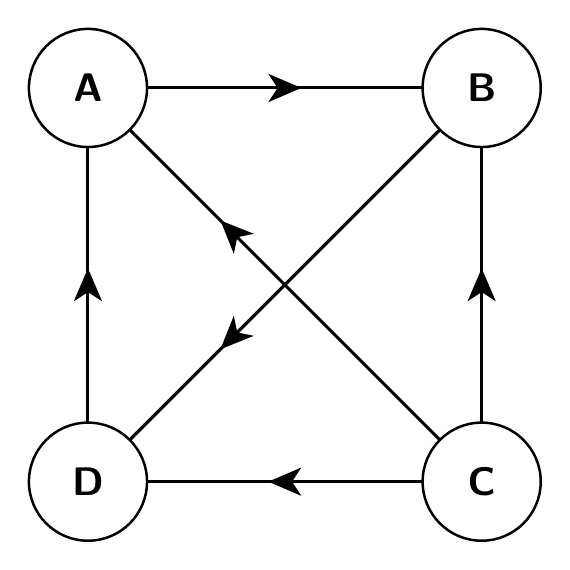
\begin{tikzpicture}[x=1cm,y=1cm]
\draw[line width=1.1pt] (4.47,0.53) -- (0.53,4.47);
\draw[line width=1.1pt] (5,0.75) -- (5,4.25);
\draw[line width=1.1pt] (4.25,0) -- (0.75,0);
\draw[line width=1.1pt] (0.75,5) -- (4.25,5);
\draw[line width=1.1pt] (4.47,4.47) -- (0.53,0.53);
\draw[line width=1.1pt] (0,0.75) -- (0,4.25);
\fill[black] (1.682,3.318) -- (1.852,2.894) -- (1.896,3.104) -- (2.106,3.148) -- cycle;
\fill[black] (5,2.71) -- (4.82,2.29) -- (5,2.408) -- (5.18,2.29) -- cycle;
\fill[black] (2.29,0) -- (2.71,-0.18) -- (2.592,0) -- (2.71,0.18) -- cycle;
\fill[black] (2.71,5) -- (2.29,5.18) -- (2.408,5) -- (2.29,4.82) -- cycle;
\fill[black] (1.682,1.682) -- (2.106,1.852) -- (1.896,1.896) -- (1.852,2.106) -- cycle;
\fill[black] (0,2.71) -- (-0.18,2.29) -- (0,2.408) -- (0.18,2.29) -- cycle;
\filldraw[fill=white, line width=0.9pt] (0,5) circle (0.75);
\node[font=\sffamily\bfseries\Large] at (0,5) {A};
\filldraw[fill=white, line width=0.9pt] (5,5) circle (0.75);
\node[font=\sffamily\bfseries\Large] at (5,5) {B};
\filldraw[fill=white, line width=0.9pt] (5,0) circle (0.75);
\node[font=\sffamily\bfseries\Large] at (5,0) {C};
\filldraw[fill=white, line width=0.9pt] (0,0) circle (0.75);
\node[font=\sffamily\bfseries\Large] at (0,0) {D};
\end{tikzpicture}
